\section {Descripción y módulos del sistema}

  \subsection{Arquitectura general}
    Para desarrollar un sistema de recomendación se han planteado los siguientes módulos funcionales de la API, el cual será utilizado por el desarrollador final para que, en conjunto con su aplicación final realice la integración de las funciones disponibles en el API junto al sistema de recomendación final. Esto se puede denotar en el diagrama de la figura~\ref{fig:architecture}

      \begin{figure}[h!]
      \centering
      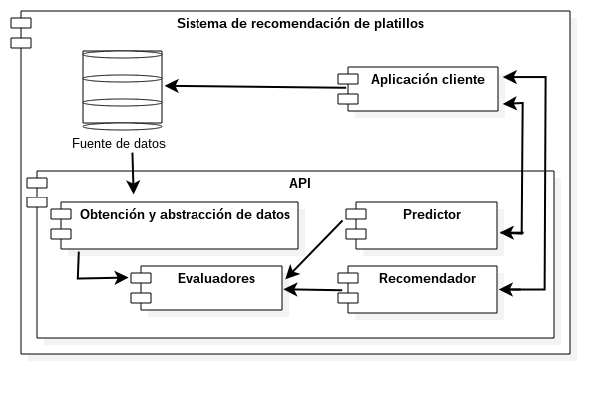
\includegraphics[width=16cm]{./images/architecture.png}
      \caption{Diagrama general del sistema}
      \label{fig:architecture}
    \end{figure}

Cómo se puede apreciar en el diagrama, el sistema se encuentra dividido en tres módulos básicos además de la aplicación final que hace uso de los módulos de la API.
    \begin{itemize}
    \item Módulo de obtención y abstracción de datos
    \item Módulo de evaluación
    \item Módulo de presentación de resultados
    \item Aplicación cliente
  \end{itemize}

\subsection{Módulos de la API}
  \subsubsection{Módulo de obtención y abstracción de datos}
    Este módulo es el encargado de la obtención de datos a través de la aplicación del caso de estudio, mapeándo dichos datos dentro de una estandarización acorde al modelo propuesto por el equipo de trabajo. Esta obtención permitirá tener la funcionalidad del sistema de recomendación de manera adecuada. 
    Se presenta como un módulo conformado por diferentes servicios proporcionados por interfaces de conexión para los datos. Tiene una interacción directa con los módulos de evaluación y presentación dentro del sistema.
    Dentro de sus características podemos denotar:
    \begin{itemize}
      \item Permite la conexión a los datos del caso de estudio.
      \item A través de interfaces, permite mapear los datos utilizados en cada caso de estudio para el correcto funcionamiento del módulo de operaciones lógicas.
      \item Se encuentra restringido al modelo de datos mínimo propuesto por el equipo de trabajo.
    \end{itemize}

  \subsubsection{Módulo de operaciones lógicas}
    El módulo de operaciones lógicas permitirá, haciendo uso de la información almacenada, obtener evaluaciones de los diferentes artículos de acuerdo a diferentes clasificaciones con base en algoritmos de recomendación que definen los principales tipos de recomendación existentes: basados en contenido, colaborativos e híbridos. Estas evaluaciones deberán ser utilizadas por el módulo de presentación de resultados para devolver predicciones o recomendaciones de los artículos utilizados por el desarrollador en su caso de estudio. Cabe destacar que este tipo de algoritmos devolverán evaluaciones cuantitativas, y la representación de estos se definirá dependiendo el caso de estudio. El uso de algoritmos con objetivos de maximización de similitud o minimización de distancia será determinado por el desarrollador. Dentro de sus características principales encontramos:
    \begin{itemize}
      \item Hace uso de la conexión proporcionada por el módulo de datos para devolver evaluaciones entre dos diferentes artículos o usuarios.
      \item Las evaluaciones son cuantitativas, denotando una distancia correspondiente a la similitud existente entre los objetos.
      \item El algoritmo de evaluación a utilizar será determinado en la interacción entre éste módulo y el módulo de presentación de resultados.
    \end{itemize}

  \subsubsection{Módulo de presentación}
    Haciendo uso del módulo de operaciones lógicas, este módulo pretende interactuar con la aplicación final para brindar las funciones de recomendación y predicción para cada usuario o artículo. Al interactual con la aplicación del caso de estudio es la via para obtener los datos a procesar y así mismo devolver una recomendación o la predicción del comportamiento de un artículo para un usuario en particular. Depende del módulo de evaluaciones para realizar el proceso lógico de la recomendación.

\subsection{Aplicación final}
  \subsubsection{Definición}
    En este caso, la aplicación final hará uso de las funciones proporcionadas por los distintos módulos que conforman la API para obtener recomendaciones de los datos que pertenezcan a su caso de estudio. Interactúa directamente con el módulo de abstracción de datos y con el módulo de presentación para hacer uso de la funcionalidad permitida por el API. En este caso, la aplicación final se verá reflejada en un sistema web que permita denotar la funcionalidad de la API para un conjunto de datos de platillos y restaurantes.